\documentclass[notheorems,hidelinks,aspectratio=1610]{beamer}
%\usetheme[compress]{JuanLesPins}
\usetheme{JuanLesPins}
\setbeamertemplate{footline}{
  \hfill%
  \usebeamercolor[fg]{page number in head/foot}%
  \usebeamerfont{page number in head/foot}%
  \setbeamertemplate{page number in head/foot}[framenumber]%
  \usebeamertemplate*{page number in head/foot}\kern1em\vskip2pt%
}
\setbeamertemplate{navigation symbols}{}
\usecolortheme{iwr}
\usepackage{mathsim}
\lstset{language=Python}
\usetikzlibrary{snakes}
\usetikzlibrary{matrix,fit}
\pgfdeclarelayer{bg}
\pgfsetlayers{bg,main}
\input{mixed/fig/tikzsettings}
\def\esp#1{V_{#1}}

\usepackage{times}
\usepackage{xr}
\externaldocument{main}
\usepackage{mfirstuc}
\usepackage{mathtools}  
\mathtoolsset{showonlyrefs}

\newcommand{\rd}{\operatorname{rd}}
\definecolor{mygreen}{RGB}{0,160,0}

\def\footnote#1{}
\def\putindex#1{#1}
\title{Differentialgleichungen}
\author{Guido Kanschat}
\date{}

\def\R{\mathbb R}
\def\Rnn{\R^{n\times n}}

\begin{document}
\frame{\maketitle}
\frame{\frametitle{Overview}\tableofcontents[hideallsubsections]}

\section{Modelierung von Populationen}
\frame{\sectoc}
\subsection{Wachstum unter Idealbedingungen}
\frame{\subtoc}
\begin{frame}{Ausgangsfragestellung}
  \begin{columns}
    \begin{column}{.6\textwidth}
      \begin{itemize}
      \item<+-> Anzucht von Hefe
      \item<+-> Fermenter
      \item<+-> Fragen:
        \begin{itemize}
        \item<+-> Wie lange muss ich warten, bis ich die gewünschte Ausbeute habe?
        \item<+-> Kann ich für einen beliebigen Zeitpunkt die Anzahl
          an Hefezellen vorhersagen?
        \end{itemize}
      \end{itemize}
    \end{column}
    \begin{column}{.39\textwidth}
      \begin{center}
        \only<2->{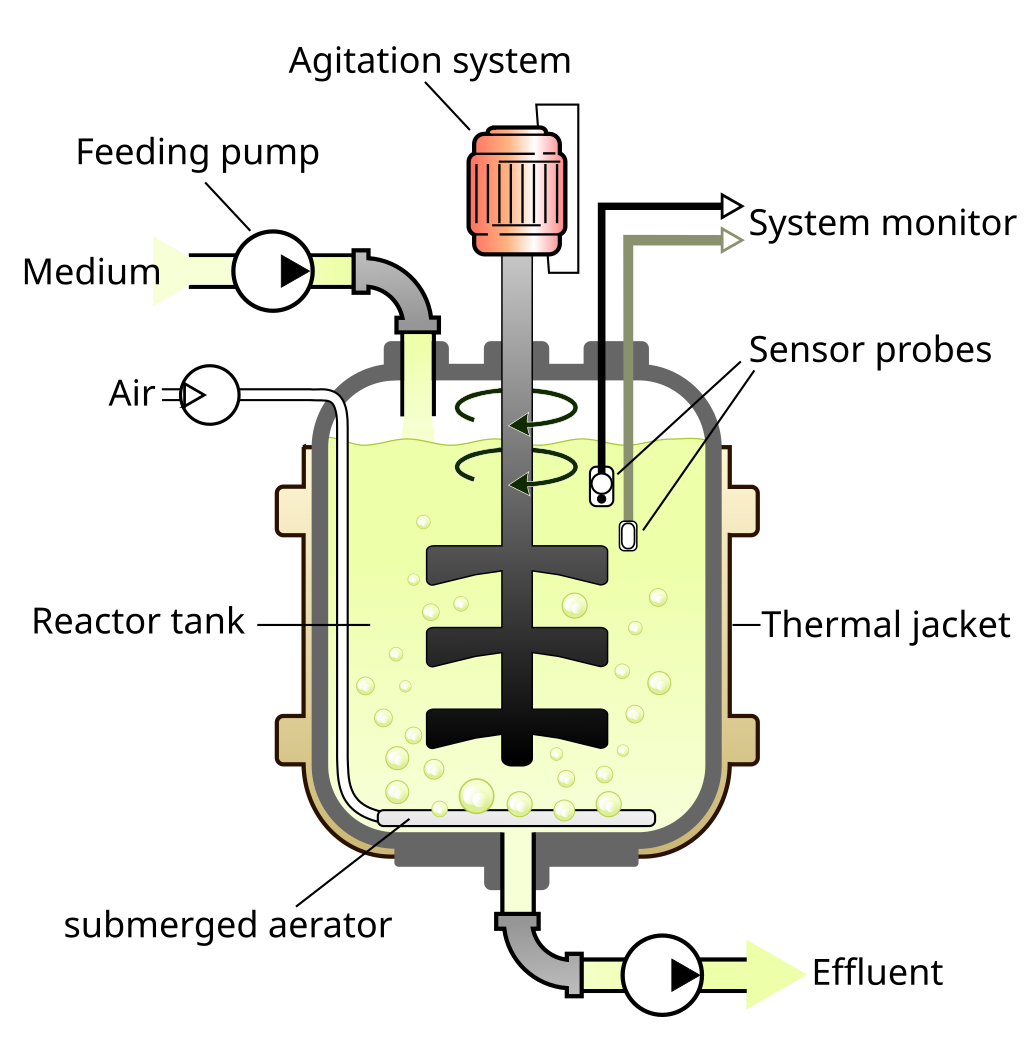
\includegraphics[width=.9\textwidth]{fig/Bioreactor}

          \tiny © Yassine Mrabet, Wikipedia
        }
      \end{center}
    \end{column}
  \end{columns}
\end{frame}

\begin{frame}
  \begin{exampleblock}{Frage}
    Welche Informationen benötigen Sie, um diese Aufgabe zu lösen?
  \end{exampleblock}
\end{frame}

\begin{frame}
  \begin{block}{Verdopplungsrate}
    Under optimal conditions, yeast cells can double their population every 100 minutes.

    \begin{flushright}
      \tiny Wikipedia: Saccaromyces cerevisiæ
    \end{flushright}
  \end{block}

  \pause
  \vspace{5mm}
  
  \begin{tikzpicture}\footnotesize
    \draw [->] (0,0) -- (12.5,0);
    \draw (0,.1)  -- (0,-.1) node[below] {8:00};
    \draw (2,.1) -- (2,-.1) node[below] {9:40};
    \draw (4,.1) -- (4,-.1) node[below] {11:20};
    \draw (6,.1) -- (6,-.1) node[below] {13:00};
    \draw (8,.1) -- (8,-.1) node[below] {14:40};
    \draw (10,.1) -- (10,-.1) node[below] {16:20};
    \draw (12,.1) -- (12,-.1) node[below] {18:00};
    \only<2>{
      \path (1,.3) node {2x};
      \path (3,.3) node {2x};
      \path (5,.3) node {2x};
      \path (7,.3) node {2x};
      \path (9,.3) node {2x};
      \path (11,.3) node {2x};
    }
    \only<3->{
      \path (0.,.1) node[above,iwrred]{1000};
      \path (2.,.1) node[above,iwrred]{2000};
      \path (4.,.1) node[above,iwrred]{4000};
      \path (6.,.1) node[above,iwrred]{8000};
      \path (8.,.1) node[above,iwrred]{16000};
      \path (10.,.1) node[above,iwrred]{32000};
      \path (12.,.1) node[above,iwrred]{64000};
    }
    \only<4>{
      \draw[mygreen] (7,.1) -- (7,-.1) node[below,mygreen] {13:50};
    }
  \end{tikzpicture}

  \pause
  \vspace{5mm}

  \begin{block}{Anfangspopulation}
    Beispiel: Die Population um 8:00 beträgt 1000 Zellen
  \end{block}
  \pause
  \begin{exampleblock}{Frage}
    Wieviele Zellen haben wir um 13:50?
  \end{exampleblock}
\end{frame}

\begin{frame}{Mathematisch etwas allgemeiner und präziser...}
  \begin{itemize}
  \item Anzahlvariable $N$
  \item Zeitvariable $t$ in Minuten, Startzeit $t_0=8:00$, ``Messzeit'' $T=18:00$
  \item Zeitintervalle $I_k = [t_{k},t_{k+1}]$ der Länge $\Delta t = 100 \text{min}$
    
    \vspace{5mm}
  \begin{tikzpicture}\footnotesize
    \draw [->] (0,0) -- (12.5,0);
    \draw (0,.1)  -- (0,-.1) node[below] {8:00};
    \draw (2,.1) -- (2,-.1) node[below] {9:40};
    \draw (4,.1) -- (4,-.1) node[below] {11:20};
    \draw (6,.1) -- (6,-.1) node[below] {13:00};
    \draw (8,.1) -- (8,-.1) node[below] {14:40};
    \draw (10,.1) -- (10,-.1) node[below] {16:20};
    \draw (12,.1) -- (12,-.1) node[below] {18:00};
      \path (0.,.1) node[above,iwrred]{1000};
      \path (1,.3) node {+1000};
      \path (3,.3) node {+2000};
      \path (5,.3) node {+4000};
      \path (7,.3) node {+8000};
      \path (9,.3) node {+16000};
      \path (11,.3) node {+32000};
    \end{tikzpicture}

    \vspace{5mm}
    
  \item Sei $d_k$ der Zuwachs im Intervall $I_k$
    \begin{gather*}
      N(t_{k+1}) = N(t_k) + d_k,
      \qquad N(T) = N(t_0) + \sum_{k=0}^{n-1} d_k.
    \end{gather*}
  \end{itemize}
  \pause
  \begin{exampleblock}{Frage}
    Im Beispiel ist $d_k=N(t_k)$. Wie ändert sich $d_k$ qualitativ, wenn wir die Intervalle halbieren?
  \end{exampleblock}
\end{frame}

\begin{frame}{Halbierung der Intervalle}

  \begin{tikzpicture}\footnotesize
    \draw [->] (0,0) -- (12.5,0);
    \draw (0,.1)  -- (0,-.1) node[below] {8:00};
    \draw (2,.1) -- (2,-.1) node[below] {9:40};
    \draw (4,.1) -- (4,-.1) node[below] {11:20};
    \draw (6,.1) -- (6,-.1) node[below] {13:00};
    \draw (8,.1) -- (8,-.1) node[below] {14:40};
    \draw (10,.1) -- (10,-.1) node[below] {16:20};
    \draw (12,.1) -- (12,-.1) node[below] {18:00};
      \path (0.,.1) node[above,iwrred]{1000};
      \path (1,.3) node {+1000};
      \path (3,.3) node {+2000};
      \path (5,.3) node {+4000};
      \path (7,.3) node {+8000};
      \path (9,.3) node {+16000};
      \path (11,.3) node {+32000};
    \end{tikzpicture}

    \vspace*{4cm}
\end{frame}

\begin{frame}{Riemannsche Summen}
  \begin{itemize}
  \item Es gilt eine Beziehung wie
    $d_k \approx f(t_k)\Delta t$.
  \item Dann können wir für eine beliebige Folge von $n$ Intervallen
    schreiben
    \begin{gather*}
      N(t_n) = N(t_0) + \sum_{k=0}^{n-1} f(t_k) (\Delta t)_k
    \end{gather*}
    \item Wenn wir die Intervalllänge gegen null gehen lassen, bekommen wir ein Integral
  \end{itemize}
  \pause
  \begin{block}{Kontinuumshypothese}
    Für individuelle Hefezellen ist $\Delta t \to 0$ unsinnig, weil sich ab einem Punkt sehr wahrscheinlich keine einzige Zelle in einem Intervall vermehrt.

    \vspace{1ex}

    Wir ersetzen daher die diskrete Anzahl $N(t)$ durch eine
    kontinuierliche Größe $x(t)$ z. B. mit der Einheit Gramm anstelle
    von Stück.
  \end{block}
\end{frame}

\begin{frame}{Integraldarstellung}
  Ersetzen wir $N(t)$ durch $x(t)$ und lassen die Summen konvergieren, so erhalten wir die Darstellung
    \begin{gather*}
      x(T) = x(t_0) + \int_{t_0}^T f(t) \dt.      
    \end{gather*}
  \begin{block}{Instantane Reproduktionsrate $R$}
    Für die Funktion unter dem Integral setzen wir
    \begin{gather*}
      f(t) = R x(t).
    \end{gather*}
    Hier repräsentiert $R$ eine Reproduktionsrate für ein unendlich kleines Zeitintervall.
    %, also
    % \begin{gather*}
    %   R = \lim_{h\to 0} \tfrac{x(t+h)-x(t)}{h}.
    % \end{gather*}
  \end{block}
\end{frame}

\begin{frame}
  Wir erhalten die Darstellung der Funktion $x(t)$ als
  \begin{block}{Volterrasche Integralgleichung}
    \begin{gather*}
      x(t) = x(t_0) + \int_{t_0}^t R x(s) \ds.      
    \end{gather*}    
  \end{block}

  Differenzieren wir auf beiden Seiten ergibt die Darstellung als
  \begin{block}{Differentialgleichung}
    \begin{gather*}
          x'(t) = R x(t)
    \end{gather*}
  \end{block}
\end{frame}

\begin{frame}{Lösungen}
  Aus der Schule ist die Exponentialfunktion bekannt. Es gilt:
  \begin{gather*}
    \tfrac d{dt} e^{Rt} = R e^{Rt}.
  \end{gather*}
  Dies gilt aber auch für alle Funktionen $x(t) = c \,e^{Rt}$ mit einer Konstanten $c$.

  \begin{block}{Anfangswertaufgabe}
    Die Lösungsgesamtheit der Differentialgleichung $x' = Rx$ besteht
    aus allen Funktionen der Form $c\,e^{Rt}$.

    \vspace{1ex}

    Die tatsächliche Lösung erhält man, indem man die Konstante an den Anfangswert $x_0$ angleicht:
    \begin{gather*}
      x_0 = x(t_0) = c e^{Rt_0} \qquad \Rightarrow \qquad c = \frac{x_0}{e^{R t_0}}
    \end{gather*}
  \end{block}
\end{frame}

\begin{frame}{Berechnung von $R$}
  Wenn $\Delta t$ die Zeit zur Verdopplung ist, wie groß ist $R$?

  \vspace{5cm}
  
\end{frame}

\begin{frame}{Einheiten}
  \begin{minipage}{.5\textwidth}
  \begin{itemize}
  \item Wir setzen Einheiten für $t$ und $x$, zum Beispiel
    \begin{gather*}
      t[\text{min}],\qquad x[\text{g}].
    \end{gather*}
  \item Dann hat $x'$ die Einheit $\nicefrac{\text{g}}{\text{min}}$
  \item Wegen
    \begin{gather*}
      R = \frac{x'}{x} \qquad\text{ist}\quad R[\nicefrac1{\text{min}}]
    \end{gather*}
  \end{itemize}    
  \end{minipage}
  \pause
  \begin{block}{Dimensionslose Formulierung}
    Indem man formal durch die Einheiten teilt, werden die Gleichungen
    dimensionslos.

    \vspace{1ex}

    Man kann auch durch charakteristische Größen teilen, um gezielt
    mathematisch einfache Darstellungen zu erhalten.
  \end{block}
\end{frame}

\begin{frame}{Asymptotische Betrachtung}
  \begin{exampleblock}{Frage}
    Was passiert, wenn Sie die Lösung der Wachstumsgleichung für immer
    größere Zeiten, also das Verhalten für $t\to\infty$ betrachten?
  \end{exampleblock}

  \begin{exampleblock}{Frage}
    Was passiert für $t\to\infty$, wenn $R<0$?
  \end{exampleblock}
\end{frame}
%%%%%%%%%%%%%%%%%%%%%%%%%%%%%%%%%%%%%%%%%%%%%%%%%%%%%%%%%%%%%%%%%%%%%% 
%%%%%%%%%%%%%%%%%%%%%%%%%%%%%%%%%%%%%%%%%%%%%%%%%%%%%%%%%%%%%%%%%%%%%%
\subsection{Einige Begriffe}
\frame{\subtoc}
\begin{frame}
  \begin{block}{Differentialgleichung}
    Eine Differentialgleichung ist eine Gleichung, die eine Funktion
    und/oder ihre Ableitungen in Beziehung setzt.
  \end{block}
  \begin{columns}
    \begin{column}[t]{.5\textwidth}
      \begin{block}{Gewöhnliche DGl.}
        Es kommen nur Ableitungen bzgl. einer Variablen vor. Beispiel:
        \begin{gather*}
          x^{(3)}(t) + \sin(t) x'(t) = x^2(t) +t^2
        \end{gather*}
      \end{block}
    \end{column}
    \begin{column}[t]{.5\textwidth}
      \begin{block}{Partielle DGl.}
        Es kommen partielle Ableitungen nach mehreren Variablen vor.
        Beispiel:
        \begin{gather*}
          \partial_t u(t,x) - \partial_{xx} u(t,x) = \sin(x)
        \end{gather*}
      [Nicht in dieser Vorlesung]
      \end{block}
    \end{column}
  \end{columns}
  \pause
  \begin{block}{Ordnung einer Differentialgleichung}
    Die Ordnung einer DGl. ist der Grad der höchsten Ableitung, die in
    der Gleichung vorkommt.
  \end{block}
\end{frame}

\begin{frame}
  \begin{block}{Autonome Differentialgleichungen}
    Eine Differentialgleichung heißt autonom, wenn keiner der Terme
    eine explizite Abhängigkeit von der Zeit hat.
  \end{block}
  \begin{columns}
    \begin{column}[t]{.5\textwidth}
      \begin{block}{Autonom}
        \begin{gather*}
          x' = f(x)
        \end{gather*}
      \end{block}
    \end{column}
    \begin{column}[t]{.5\textwidth}
      \begin{block}{Nicht autonom}
        \begin{gather*}
          x' = f(t,x)
        \end{gather*}
      \end{block}
    \end{column}
  \end{columns}
  \pause Konsequenz: bei autonomen DGln. ist der Startzeitpunkt frei
  verschiebbar, wir wählen oft $t_0 = 0$.
  \begin{exampleblock}{Frage}
    Welche Prozesse führen zu autonomen DGln., welche zu nicht autonomen?
  \end{exampleblock}
\end{frame}

\begin{frame}
  \begin{block}{Homogene Differentialgleichungen}
    Eine Differentialgleichung ist homogen, wenn es keinen Summanden
    gibt, der die Lösungsfunktion nicht enthält. Einen solchen
    Summanden nennt man dann die Inhomogenität.
  \end{block}
  \begin{columns}
    \begin{column}[t]{.5\textwidth}
      \begin{block}{Homogen}
        \begin{gather*}
          x'+ \sin(t) x = 0
        \end{gather*}
      \end{block}
    \end{column}
    \begin{column}[t]{.5\textwidth}
      \begin{block}{Nicht homogen}
        \begin{gather*}
          x'+ \sin(t) x = 5
        \end{gather*}
      \end{block}
    \end{column}
  \end{columns}
  \begin{exampleblock}{Frage}
    Welche Prozesse führen zu homogenen DGln., welche zu nicht homogenen?
  \end{exampleblock}
\end{frame}

%%%%%%%%%%%%%%%%%%%%%%%%%%%%%%%%%%%%%%%%%%%%%%%%%%%%%%%%%%%%%%%%%%%%%%
%%%%%%%%%%%%%%%%%%%%%%%%%%%%%%%%%%%%%%%%%%%%%%%%%%%%%%%%%%%%%%%%%%%%%%
\subsection{Wachstum bei begrenzter Nahrung}
\frame{\subtoc}

\begin{frame}
  \begin{exampleblock}{Frage}
    Was erwarten Sie im Fermenter, wenn Sie im Prozess keine Nahrung
    zuführen? Betrachten Sie vor allem den Fall $t\to\infty$.
  \end{exampleblock}
\end{frame}

\begin{frame}
  \begin{exampleblock}{Frage}
    Was erwarten Sie im Fermenter, wenn Sie im Prozess mit konstanter
    Rate Nahrung zuführen? Betrachten Sie vor allem den Fall
    $t\to\infty$.
  \end{exampleblock}
\end{frame}

\begin{frame}{Modellierung}
  \begin{itemize}
  \item Bisher hatten wir $R$ bei optimalen Bedingungen (Nahrungsmenge
    $F_{\text{opt}}$)
  \item Bei Nahrungszufuhr $F_{\text{opt}}$ ist der Anteil an verfügbarer Nahrung $1-Vx$, wobei $Vx$ der Verbrauch der Hefe ist.
  \item Jetzt setzen wir unter Vereinfachung für die Reproduktionsrate
    \begin{gather*}
      r = R \frac{F}{F_{\text{opt}}} = R (1-Vx)
    \end{gather*}
  \item Wir erhalten die ``logistische Differentialgleichung''
    \begin{gather*}
      x' = rx = R (1-Vx) x.
    \end{gather*}
  \end{itemize}
\end{frame}

\begin{frame}
  \begin{block}{Lösungen}
    \begin{gather*}
      x_c(t) = \frac{e^{Rt}}{V e^{Rt}+c}
    \end{gather*}
  \end{block}
\end{frame}

\begin{frame}{Richtungsfelder}
  \begin{columns}
    \begin{column}[t]{.2\textwidth}
    \begin{gather*}
      x'= (1-x) x
    \end{gather*}
    \begin{exampleblock}{Frage}
      Verhalten für $t\to\infty$
    \end{exampleblock}
    \end{column}
    \begin{column}[t]{.8\textwidth}
      \mbox{}
      
      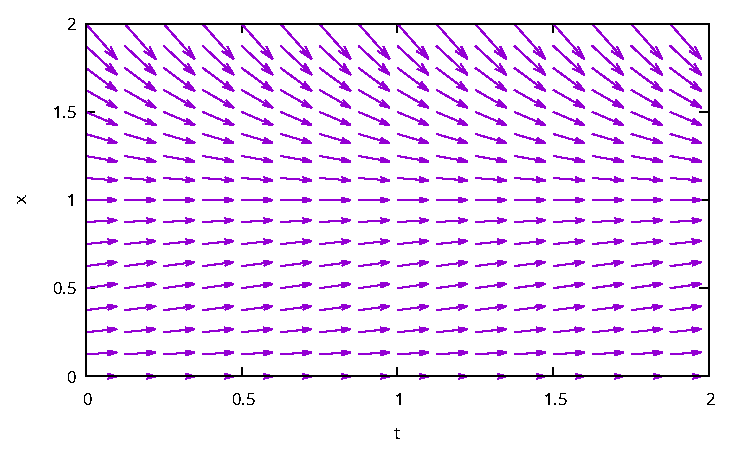
\includegraphics[width=\textwidth]{gnuplot/logistic.pdf}
    \end{column}
  \end{columns}
\end{frame}

\begin{frame}{Negative Startwerte}
  \begin{columns}
    \begin{column}[t]{.2\textwidth}
    \begin{gather*}
      x'= (1-x) x
    \end{gather*}      
    \end{column}
    \begin{column}[t]{.8\textwidth}
      \mbox{}
      
      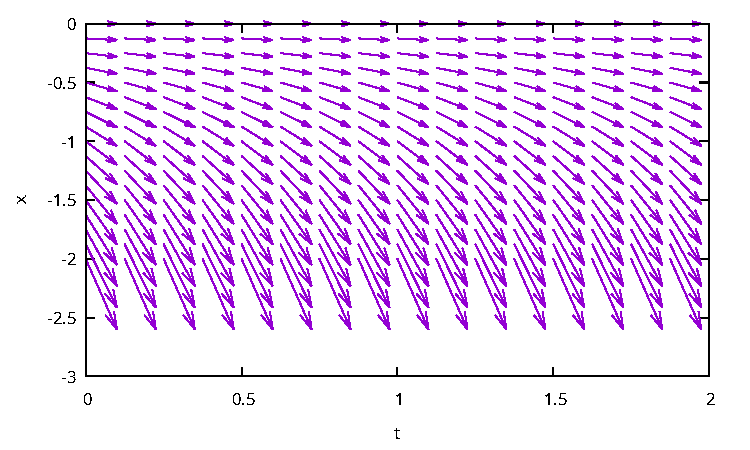
\includegraphics[width=\textwidth]{gnuplot/logisticm.pdf}
    \end{column}
  \end{columns}
\end{frame}

\begin{frame}{Fixpunkte}
  \begin{columns}
    \begin{column}{.1\textwidth}
      \mbox{}
      
      \begin{tikzpicture}[scale=1.]]
        \node (A) at (0,0) {$\bullet$};
        \node (B) at (0,1) {$\bullet$};
        \node (C) at (0,-2) {};
        \node (D) at (0,3) {};

        \draw[thick,-Stealth] (A) edge (B);
        \draw[thick,-Stealth] (A) edge (C);
        \draw[thick,-Stealth] (D) edge (B);
      \end{tikzpicture}
    \end{column}
    \pause
    \begin{column}{.9\textwidth}
      Für autonome Gleichungen sind Fixpunkte von hoher Bedeutung. Es gilt:
      \begin{gather*}
        x'(T) = 0 \qquad \Rightarrow \qquad x(t) = 0
        \quad\text{für alle}\quad t>T
      \end{gather*}

      Es gibt
      \begin{itemize}
      \item anziehende Fixpunkte: Richtungspfeile zeigen zum Fixpunkt hin
      \item abstoßende Fixpunkte: Richtungspfeile zeigen vom Fixpunkt weg
      \item gemischte Fixpunkte
      \end{itemize}
    \end{column}
  \end{columns}
\end{frame}

\begin{frame}
  \begin{exampleblock}{Frage}
    Wie finden Sie bei einer autonomen Differentialgleichung der Form
    \begin{gather*}
      x' = f(x)
    \end{gather*}
    alle Fixpunkte?
  \end{exampleblock}
  \pause
  \begin{exampleblock}{Frage}
    Woran erkennen Sie, ob diese Fixpunkte anziehend oder abstoßend sind?
  \end{exampleblock}
\end{frame}

\begin{frame}{Charakterisierung von Fixpunkten}
  Bei einer Gleichung erster Ordnung der Form
    \begin{gather*}
      x' = f(x)
    \end{gather*}
    sind die Fixpunkte die Nullstellen der Funktion $f$.
\end{frame}
  
%%%%%%%%%%%%%%%%%%%%%%%%%%%%%%%%%%%%%%%%%%%%%%%%%%%%%%%%%%%%%%%%%%%%%%
%%%%%%%%%%%%%%%%%%%%%%%%%%%%%%%%%%%%%%%%%%%%%%%%%%%%%%%%%%%%%%%%%%%%%%
\subsection{Das Räuber-Beute-Modell}
\frame{\subtoc}

\begin{frame}{Erweiterung auf zweite Species}
  \begin{itemize}
  \item Sardinen finden optimale Nahrung und werden von
    Thunfischen gefressen
  \item Thunfisch frisst Sardinen und stirbt eines natürlichen
    Todes
  \end{itemize}
  \pause
  Wir wollen möglichst einfache Beziehungen annehmen!
  \begin{exampleblock}{Aufgabe}
    Überlegen Sie sich, wie Sie die Entwicklung der Populationen
    modellieren könnten!
  \end{exampleblock}
\end{frame}

\begin{frame}{Modellierung}
  \begin{itemize}
  \item<+-> Sardinen:
    \begin{itemize}
    \item Vermehrung mit fester Rate: $ax$
    \item Sterberate abhängig vom Thunfisch: $-bxy$
    \end{itemize}
    \begin{gather*}
      x' = ax-bxy
    \end{gather*}
  \item<+-> Thunfisch:
    \begin{itemize}
    \item Feste Sterberate: $-cy$
    \item Vermehrung abhängig von Sardinen: $dxy$
    \end{itemize}
    \begin{gather*}
      y' = -cy + dxy
    \end{gather*}
  \item<+-> $a,b,c,d$ sind angenommene, feste Parameter
  \end{itemize}
\end{frame}

\begin{frame}{Lotka-Volterra-Gleichungen}
  \begin{gather*}
    \begin{aligned}
      x' &=& ax &-bxy\\
      y' &=& -cy & +dxy
    \end{aligned}
  \end{gather*}

  \begin{block}{System von Differentialgleichungen}
    Mehrere Differentialgleichungen für mehrere Funktionen bilden ein
    System von DGln. Die Anzahl der Gln./Funktionen ist die Dimension
    des Systems.
  \end{block}
\end{frame}

\begin{frame}{Phasenraumdiagramme}
  \begin{itemize}
  \item Die Lotka-Volterra-Gleichungen sind autonom
    \begin{itemize}
    \item[$\Rightarrow$] die Entwicklung hängt nur von $(x,y)$ ab 
    \end{itemize}
  \item Man bezeichnet den Raum der möglichen Zustände als Phasenraum
  \item Auch dort können wir wieder Richtungsfelder zeichnen
  \end{itemize}
\end{frame}

\begin{frame}{Richtungsfeld im Phasenraum}
  \begin{center}
    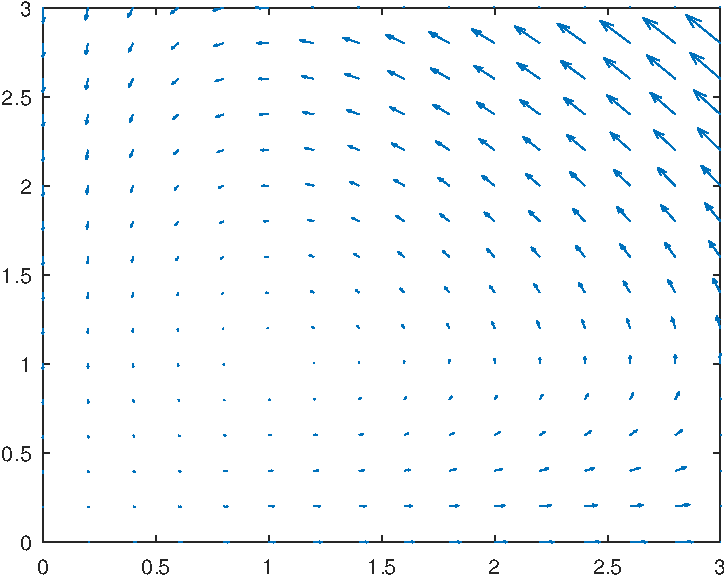
\includegraphics[width=.7\textwidth]{octave/volterra-vectors-crop.pdf}
  \end{center}
\end{frame}

\begin{frame}{Lösung im Phasenraum}
  \begin{center}
    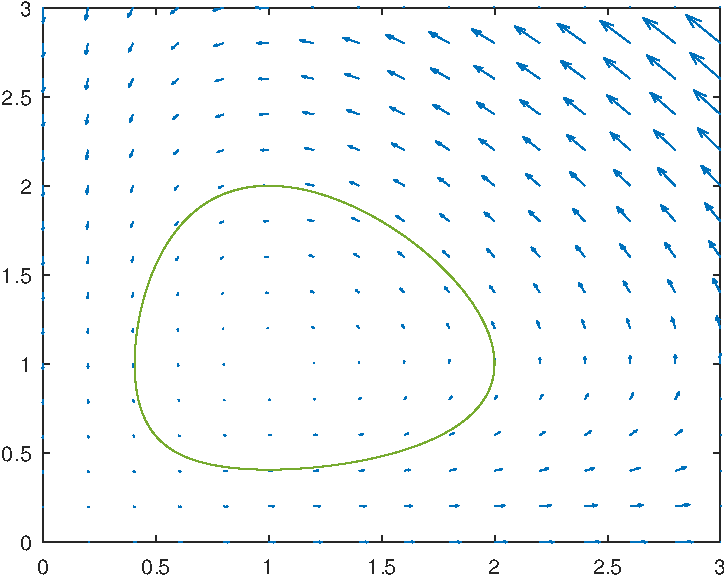
\includegraphics[width=.7\textwidth]{octave/volterra-phasespace-crop.pdf}
  \end{center}  
\end{frame}

\begin{frame}{Lösung als Funktion der Zeit}
  \begin{center}
    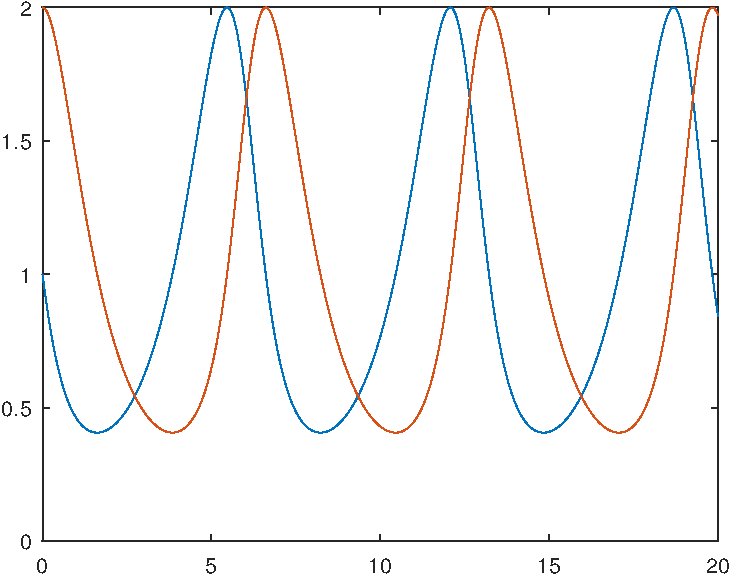
\includegraphics[width=.7\textwidth]{octave/volterra-timeseries-crop.pdf}
  \end{center}  
\end{frame}

\begin{frame}
  \begin{block}{Warnung}
    Für die Lotka-Volterra-Gleichungen gibt es keine geschlossene
    Darstellung der Lösungen.
  \end{block}

  Es lassen sich aber einige Aussagen treffen
  \begin{itemize}
  \item Es gibt die beiden Fixpunkte $(0,0)^T$ und
    $\left(\tfrac cd,\tfrac ab\right)^T$
  \item Lösungen sind periodisch
  \item Es gibt diverse Erhaltungssätze
  \end{itemize}
\end{frame}

\begin{frame}{Lösungen zu verschiedenen Anfangswerten}
  \begin{center}
    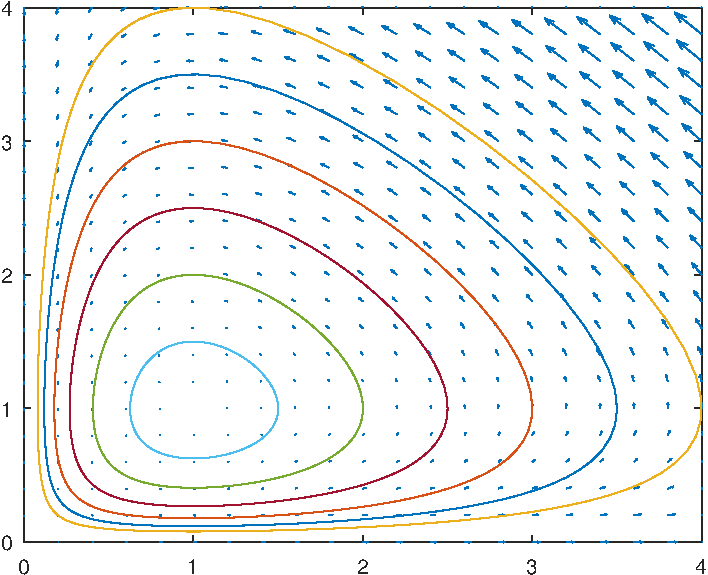
\includegraphics[width=.7\textwidth]{octave/volterra-multi-crop.pdf}
  \end{center}    
\end{frame}

%%%%%%%%%%%%%%%%%%%%%%%%%%%%%%%%%%%%%%%%%%%%%%%%%%%%%%%%%%%%%%%%%%%%%%
%%%%%%%%%%%%%%%%%%%%%%%%%%%%%%%%%%%%%%%%%%%%%%%%%%%%%%%%%%%%%%%%%%%%%%
\subsection{Zusammenfassung}
\frame{\subtoc}

\begin{frame}{Zusammenfassung Modellierung}
  \begin{enumerate}
  \item Unter Annahme der Kontinuumshypothese können wir
    Wachtumsprozesse durch Differentialgleichungen
    beschreiben.
  \item Populationsdynamik mehrerer Spezies führt zu Systemen von DGln.
  \item Diese DGLn. haben unendlich viele Lösungen, was uns eigentlich interessiert, ist die Lösung einer Anfangswertaufgabe (AWA)
  \item Das Ergebnis der eigentlichen Modellierung war die
    Volterrasche Integralgleichung
  \end{enumerate}
\end{frame}

\begin{frame}{Zusammenfassung Analyse}
  \begin{enumerate}
  \item Qualitative Diskussion zum Verständnis der Modelle
    \begin{itemize}
    \item Richtungsfelder
    \item Phasenraumdiagramme
    \end{itemize}
  \item Verhalten für große Zeiten
    \begin{itemize}
    \item Fixpunkte
    \end{itemize}
  \item Wir haben die allgemeine Lösung der DGl. geraten und an den
    Anfangswert angeglichen
  \end{enumerate}
\end{frame}


\section{Berechnung von Lösungen}
\frame{\sectoc}

%%%%%%%%%%%%%%%%%%%%%%%%%%%%%%%%%%%%%%%%%%%%%%%%%%%%%%%%%%%%%%%%%%%%%%
\subsection{Lineare Systeme von Differentialgleichungen}
\frame{\subtoc}

\begin{frame}
  \begin{block}{Lineares System von Differentialgleichungen}
    Ein lineares System von DGl. erster Ordnung der Dimension $n$ hat
    die Form
    \begin{gather*}
      x' = Ax + f
      \qquad\text{oder}\qquad
      x'(t) = A(t)x(t) + f(t)
    \end{gather*}
    Es sind $x(t), x'(t), f(t) \in \R^n$ und $A(t)\in \Rnn$.
    
    Falls $A$ und $f$ nicht von der Zeit $t$ abhängen, ist das System
    autonom, es ist homogen, falls $f\equiv0$.
  \end{block}

  \begin{block}{Lösung der AWA im homogenen, autonomen Fall}
    Wie im Falle der linearen Wachstumsgleichung schreiben wir die
    Lösung der Anfangswertaufgabe mit einem Startvektor $x(0) = x_0\in\R^n$:
    \begin{gather*}
      x(t) = e^{At} x_0.
    \end{gather*}
  \end{block}
\end{frame}

\begin{frame}{Exponentialfunktion einer Diagonalmatrix}
\end{frame}

\begin{frame}{Exponentialfunktion einer diagonalisierbaren Matrix}
  
\end{frame}

\begin{frame}{Eigenschaften der Matrix-Exponentialfunktion}
  Für beliebige Matrizen $A$ und invertierbare Matrizen $S$ gilt
  \begin{align*}
    e^0 &= \mathbb I\\
    e^{S^{-1}AS} &= S^{-1} e^A S\\
    e^{\alpha A} e^{\beta A} &= e^{(\alpha+\beta) A}\\
    e^{A}e^{-A} &= \mathbb I\\
  \end{align*}
  \begin{itemize}
  \item Aus der letzten Gleichung folgt insbesondere, dass $e^A$ für jede
    Matrix $A$ invertierbar ist und $e^{-A}$ die Inverse ist.
  \item Aus der zweiten Eigenschaft folgt, dass die Eigenvektoren von
    $e^A$ identisch mit denen von $A$ sind.
  \end{itemize}
\end{frame}

\begin{frame}{Beispiel}
  \begin{gather*}
    A =
    \begin{pmatrix}
      0 & 1\\k^2 & 0
    \end{pmatrix},
    \qquad \lambda_{1/2} = \pm k,
    \qquad v_1 =
    \begin{pmatrix}
      1\\k
    \end{pmatrix},
    \quad
    v_2 =
    \begin{pmatrix}
      1 \\ -k
    \end{pmatrix}.
  \end{gather*}
  \pause
  Sei $S$ die Matrix mit Spalten $v_1$ und $v_2$, dann gilt
  \begin{gather*}
    A = S^{-1}
    \begin{pmatrix}
      k \\ &-k
    \end{pmatrix}
    S,
    \qquad
    S^{-1} =
    \frac12
    \begin{pmatrix}
      1 & \tfrac1k\\
      1 & -\tfrac1k\\
    \end{pmatrix}
  \end{gather*}
  \pause
  Nun exponenzieren wir die Eigenwerte und erhalten
  \begin{gather*}
    e^A =  S^{-1}
    \begin{pmatrix}
      e^k \\ &e^{-k}
    \end{pmatrix}
    S
    = \frac12
    \begin{pmatrix}
      e^k + e^{-k} & \tfrac 1k (e^k - e^{-k}) \\
      k (e^k - e^{-k}) & e^k + e^{-k}
    \end{pmatrix}
    =
    \begin{pmatrix}
      \cosh(k) & \tfrac 1k \sinh(k) \\
      k \sinh(k) & \cosh(k)
    \end{pmatrix}
  \end{gather*}
  \vspace*{.9\textheight}
\end{frame}

\begin{frame}{Lösung des allgemeinen linearen Systems}
  \begin{block}{Integrierender Faktor}
    Zum System
    \begin{gather*}
      x'(t) = A(t) x(t) + f(t)
    \end{gather*}
    definieren wir den integrierenden Faktor
    \begin{gather*}
      M(t) = \exp\left(-\int_0^t A(s) \,ds\right).
    \end{gather*}
  \end{block}
  Wir beobachten, dass
  \begin{align*}
    M(0) &= \mathbb I,\\
    M'(t) &= -M(t) A(t).
  \end{align*}
\end{frame}

\begin{frame}
  \begin{block}{Lösung mit integrierendem Faktor}
    Für die Anwangswertaufgabe
    \begin{gather*}
      x'(t) = A(t)u(t)+ f(t),
      \qquad
      x(0) = x_0,
    \end{gather*}
    lässt sich die Lösung mit dem integrierenden Faktor $M(t)$ über die Formel
    \begin{gather*}
      x(t) = M^{-1}(t)
      \left(
        x_0 + \int_0^t M(s) f(s) \,ds
      \right)
    \end{gather*}
    darstellen.
  \end{block}
\end{frame}

\begin{frame}
  \begin{block}{Lösungsraum}
    Die Lösungen des homogenen, linearen Systems der Dimension $n$
    \begin{gather*}
      x'(t) = A(t)x(t)
    \end{gather*}
    bilden einen Vektorraum der Dimension $n$
  \end{block}
  \pause
  Begründung:
  \begin{enumerate}
  \item Mit zwei Lösungsfunktionen $x_1$ und $x_2$ ist auch
    $ax_1+bx_2$ eine Lösung
  \item Aufgrund der Invertierbarkeit der Exponentialfunktion bildet
    \begin{gather*}
      x_1 = M^{-1} e_1, x_2 = M^{-1} e_2,\dots, x_n = M^{-1} e_n,
    \end{gather*}
    mit der Einheitsbasis $e_1,\dots,e_n$ eine Basis.
  \end{enumerate}
\end{frame}

\begin{frame}{Fixpunkte}
  \begin{gather*}
    x' = Ax+f
  \end{gather*}
  \begin{exampleblock}{Frage}
    Welche Bedingung stellen Sie an einen Fixpunkt des Systems?
  \end{exampleblock}
\end{frame}


\begin{frame}{Fixpunkte}
  \begin{block}{Satz}
  Das autonome System
  \begin{gather*}
    x' = Ax+f
  \end{gather*}
  hat unter der Bedingung, dass $A$ invertierbar ist, genau einen Fixpunkt
  \begin{gather*}
    x_F = -A^{-1}f.
  \end{gather*}
  Das Spektrum von $A$ entscheidet dabei über den Charakter des Fixpunkts.    
  \end{block}
\end{frame}


\begin{frame}{Beispiele}
  \begin{center}
    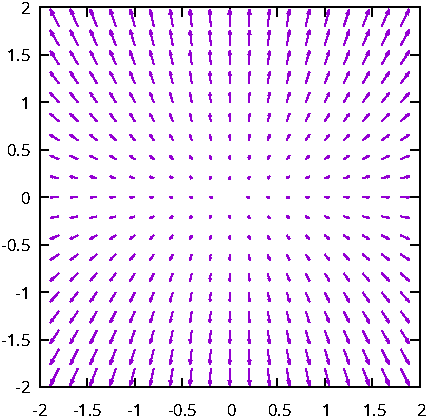
\includegraphics[width=.32\textwidth]{gnuplot/linear-pp-crop.pdf}
    \hfill
    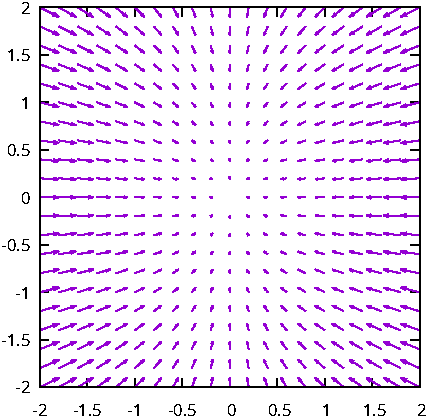
\includegraphics[width=.32\textwidth]{gnuplot/linear-mm-crop.pdf}
    \hfill
    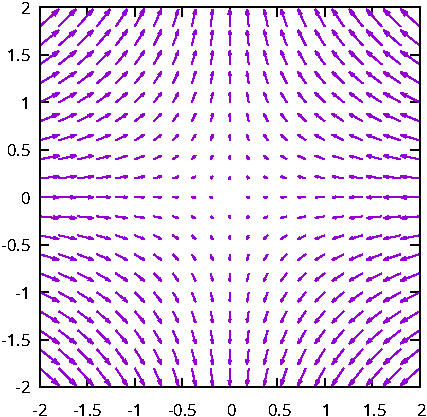
\includegraphics[width=.32\textwidth]{gnuplot/linear-pm-crop.pdf}
  \end{center}
\end{frame}

\begin{frame}
  \begin{exampleblock}{Diskussion}
    Reelle Matrizen können komplexe Eigenwerte haben. Offensichtlich
    wollen wir aber keine komplexwertigen Lösungen unserer AWA.
  \end{exampleblock}
\end{frame}

\begin{frame}{Komplexe Eigenwerte}
  \begin{block}{Satz}
    Hat eine reelle Matrix komplexe Eigenwerte, so treten sie als
    komplex konjugierte Paare mit ebensolchen Paaren von Eigenvektoren
    auf.
  \end{block}
  \pause
  Sei nun $r\pm i\phi$ ein solches Paar mit den Eigenvektoren $u\pm iv$
  \begin{align*}
    A (u\pm iv) &= {r+i\phi} (u\pm iv),\\
    e^A (u\pm iv) &= e^{r+i\phi} (u\pm iv) = e^r (\cos\phi \pm i \sin\phi)(u\pm iv).
  \end{align*}

  \vspace*{4cm}
\end{frame}

\begin{frame}
  \begin{block}{Reelle Lösungen}
    Hat die Matrix $A$ ein komplexes Eigenwertpaar
    $\lambda_{1/2} = r\pm i\phi$ mit zugehörigen Eigenvektoren
    $u\pm iv$, so ersetzen wir in der Transformationsmatrix die
    Eigenvektoren durch $u$ und $v$ und erhalten für $e^A$ eine
    quasi-Diagonalmatrix mit Block
    \begin{gather*}
      e^r
      \begin{pmatrix}
        \cos\phi & \sin\phi\\
        -\sin\phi & \cos \phi
      \end{pmatrix}
    \end{gather*}
  \end{block}
\end{frame}

\begin{frame}{Beispiele}
  \begin{center}
    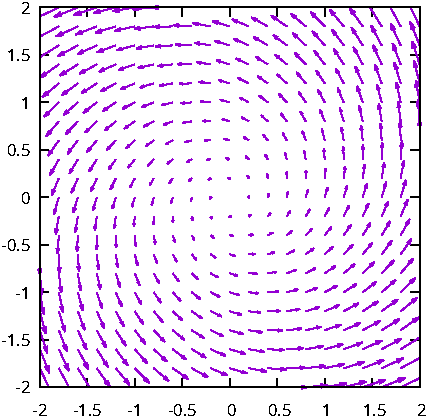
\includegraphics[width=.32\textwidth]{gnuplot/linear-cp-crop.pdf}
    \hfill
    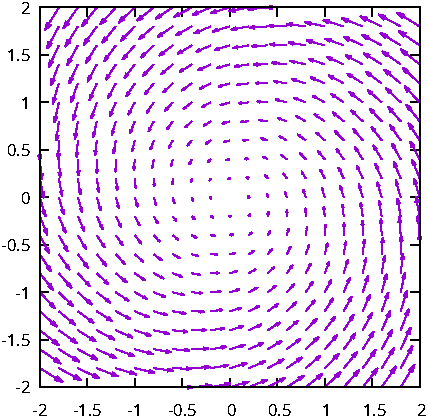
\includegraphics[width=.32\textwidth]{gnuplot/linear-cm-crop.pdf}
    \hfill
    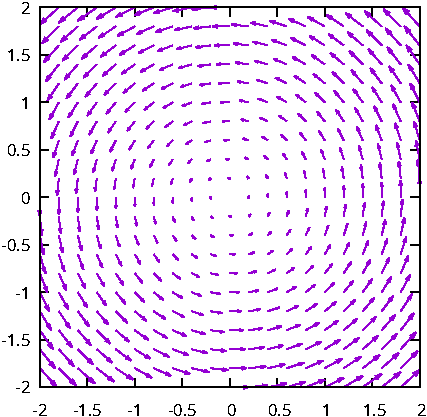
\includegraphics[width=.32\textwidth]{gnuplot/linear-c0-crop.pdf}
  \end{center}  
\end{frame}

%%%%%%%%%%%%%%%%%%%%%%%%%%%%%%%%%%%%%%%%%%%%%%%%%%%%%%%%%%%%%%%%%%%%%%
\subsection{Separable Gleichungen}
\frame{\subtoc}

\begin{frame}{Separation der Variablen}
  \begin{block}{Separable Gleichung}
    Eine DGl. der Form
    \begin{gather*}
      \frac{dx}{dt} = f(x)g(t)
    \end{gather*}
    heißt separabel.
  \end{block}

  \pause
  \begin{block}{Separationsansatz}
    \begin{enumerate}
    \item Schreibe die Gleichung in der Form
      \begin{gather*}
        \int \frac{dx}{f(x)} = \int g(t) \,dt.
      \end{gather*}
    \item Berechne beide Integrale
    \item Löse nach $x$ auf
    \end{enumerate}
  \end{block}
\end{frame}

\begin{frame}{Beispiel}
  \begin{gather*}
    x' = 2tx
  \end{gather*}
  \pause
  \begin{gather*}
    \int \frac1x\,dx = \int 2t \,dt
  \end{gather*}
  \pause
  \begin{gather*}
    \ln(x-c) = t^2
  \end{gather*}
  \pause
  \begin{gather*}
    x = e^{t^2}+c
  \end{gather*}
\end{frame}

%%%%%%%%%%%%%%%%%%%%%%%%%%%%%%%%%%%%%%%%%%%%%%%%%%%%%%%%%%%%%%%%%%%%%%
\subsection{Praktische Berechnung von Lösungen}
\frame{\subtoc}

\begin{frame}{Lösungen im Netz}
  Das Internet bietet uns viele Möglichkeiten zur Lösung von
  Differentialgleichungen
  \begin{itemize}
  \item Wikipedia
  \item Wolfram Alpha
  \item Suchfunktionen
  \item Generative KI
  \item Computeralgebrasysteme (CAS)
  \end{itemize}
\end{frame}

\begin{frame}{Kontrolle der Lösung}
  \begin{itemize}
  \item Das Lösen einer Differentialgleichung auf analytischem Wege mit
  \glqq{}Papier und Bleistift\grqq{} ist aufwändig und involviert
  schwierige Integrale.
\item Die Kontrolle, ob eine Lösung korrekt ist, erfordert nur das
  Gleichsetzen von Ableitungen. Dies ist einfach und stellt sicher,
  dass man selbst oder das Hilfsmittel korrekt gerechnet hat.
  \end{itemize}
\end{frame}

\section{Numerische Verfahren}
\frame{\sectoc}

\section{Qualitative Betrachtungen}
\frame{\sectoc}



\end{document}

%%% Local Variables:
%%% mode: latex
%%% TeX-master: t
%%% End:
